%insert blank page
\newpage\null\pagestyle{plain}\newpage

% header with section title
\pagestyle{fancy}
\fancyhf{}
\renewcommand{\sectionmark}[1]{\markright{#1}} %no number
\fancyhead[le,ro]{\nouppercase{\rightmark}}
\fancyfoot[le,ro]{\thepage}
\renewcommand{\headrulewidth}{.4pt}
\renewcommand{\footrulewidth}{.4pt}

%!TEX root = ../dissertation.tex
\begin{savequote}[82mm]
If the human brain were so simple that we could understand it, we would be so simple that we couldn’t.
\qauthor{Emerson M. Pugh}
\end{savequote}

\chapter{Discussion}
The general objective of this dissertation was to facilitate an understanding of the complex processes surrounding transcriptional interactions in mammalian cells. The multi-leveled relationships of only two interacting molecule species make analysis and interpretation inaccessible without the help of software, and even the output of software analyses can be overwhelming in the multitude of genes that are involved. Additionally, while this dissertation started with the objective of illuminating cholinergic processes exclusively in neurons, it naturally gravitated towards immunology in all of the different foci: the studied degenerative and non-degenerative psychiatric diseases, as well as stroke, all have significant immunological components. Arguably, immune cells and the central nervous system are those two mammalian tissues that offer the greatest challenges to the life sciences in terms of complexity. 

Historically, the areas of immunology and neuroscience research have little in common, and translational advances have been few. However, as Robert Dantzer illustrates in his recent review,\cite{Dantzer2018} the two disciplines have much to learn from each other, and bringing them closer together is all but necessary. Not by coincidence, the description of brain-to-immune-signalling in that review is predominated by cholinergic implications in immunity; and the best-studied immune-to-brain-signalling molecules are the endogenous pyrogens IL-1$\upbeta$, IL-6, TNF-$\upalpha$, and IFN-$\upalpha$, which in this dissertation also are frequently implicated. However, current research barely scratches the surface of neuro-immune communication; currently, interactions are mainly studied at the level of cell-to-cell or pro"-tein-to-pro"-tein (also including transcriptional processes induced by proteins). An enormous amount of transcriptional interactions are still almost completely in the dark, including but not limited to small RNA regulatory processes. The main challenge in adding an additional regulatory layer onto an already complex subject such as neuro-immune communication is the resulting exponential increase in complexity.

This brings us back to the initial objective of this dissertation, the facilitation of an understanding of transcriptional interactions. Since the data generated by modern life-science technologies is not comprehensible to humans in its raw form, and even after statistical analyses often remains overwhelming, dimensionality reduction is a logical step to further the comprehension of the science by the scientist. Indeed, most approaches described in this dissertation result in reduction of dimensionality, and a common train of thought behind the distinct analysis steps undertaken was governed by the idea of a »smart« dimensionality reduction, as opposed to, for instance, exclusively looking at the miRNA$\to$gene relationship with the lowest p-value.

To this end, I had to develop a computational basis for the assessment of transcriptional interactions in a manner that is practicable in day-to-day research, i.e., that can generate results for these complex interactions in a matter of seconds to hours. I also had the fortune to be able to apply these methods to a range of relevant biological data, including the ones discussed in-depth in this dissertation: the cellular model of human male and female cholinergic neurons, and the blood of stroke patients. All undertaken analyses are subject to a wide variety of limitations, the most important of which will be discussed in the following.

For the sake of clarity, the discussion will be split into parts: first, the methodological and technical aspects; second, the bio-mechanistic perspective and basic molecular biology implications; and third, the physiologic, pathologic, and medical/therapeutic inferences.

%!TEX root = ../dissertation.tex
\section{Methods} \label{sec:discussion:methods}

\subsection{Transcriptional Interactions: \emph{miRNeo}} \label{sec:discussion:mirneo}
The comprehensive (however justified this term may be) analysis of transcriptional interactions seems to be, for the moment, a rather marginal endeavour. At the beginning of my work on this dissertation, a database such as \emph{miRNeo}, even in its most basic form, was not available. Recently, some efforts have been published,\cite{Fan2016, Tokar2018} including one which has necessitated a name change of my database, which was previously called \emph{miRNet}.\cite{Lobentanzer2019a, Fan2016} The premise of the approach is simple: for a biological network that is structured in the way of interaction partners connected by molecular interactions, build a database that models interaction partners as nodes of a network, and their interactions as its edges (see Chapter 2). The technical implementations, however, diverge.

\emph{miRNeo} follows the philosophy of modelling the studied networks as closely as possible in the raw database, to keep data recall at a minimum in terms of storage and processing power requirements. Neo4j seemed like a fitting platform for its implementation, since it is focused around building large networks with flexible computational requirements and possesses an infrastructure for process optimisation. Additionally, it can be integrated into development environments common in bioinformatics, such as Java and R. Most of the work presented in this dissertation has been performed on Neo4j version 3.0, however, the release of Neo4j version 4.0 was just announced and promises to bring further improvement in terms of handling and performance.\cite{Neo4j2020}

The main drawback of graph database integration into biological applications is the difference in infrastructure to virtually all other data, which is in tabular format. The effort of transitioning data into a dedicated graph format is not justified for simple questions, such as the gene targets of a single miRNA. The practical creation of \emph{miRNeo} from raw data in its current extent, without accounting for development time, would take up the majority of a month in computational time on a standard 16-core personal computer. However, nested analyses with multiple levels, and dynamic analyses with multiple steps in which the analysis in the next step depends on the result of the previous, necessitate computationally efficient implementation, and \emph{miRNeo} was able to handle all complex questions that presented themselves during my work. The most computationally demanding questions were the comprehensive whole-genome feedforward loop analyses (Section \ref{sec:stroke:ffl}), which nevertheless were completed in a matter of hours.

The most important limitation of \emph{miRNeo} is the sum of limitations that apply to the raw data \emph{miRNeo} is created from. Small RNA targeting is immensely complex, and small RNA expression is even more tissue-specific than transcription factor expression.\cite{Nowakowski2018} Thus, all results from predictions, be they based on complementarity, evolutionary conservation, or physical modelling, and even experimentally validated interactions can currently not be seen as certain indications of an actual interaction in different contexts, making validations indispensable. However, complex multi-layer interactions are nearly impossible to validate, making this area of research highly dependent on inferral from circumstantial evidence. In 2017, Kenneth Kosik introduced an experimental model of miRNA interactions at a conference for non-coding RNA in neurodegenerative disease.\cite{Kosik2017p} The study included the successive knockout of each one of a set of 11 miRNAs and observation of the cellular phenotype for each of the resulting cultures in a high throughput setting; he gave the cost of these experiments to be in the million dollar range. According to Kosik, the knockout of \emph{each one} of the 11 miRNAs led to a loss of the particular phenotype, which implied that all 11 cooperated to govern the molecular basis of the phenotype. However, this kind of experimentation cannot be applied to all open questions simply for economical reasons, and additionally, there still has been no publication of the study in a peer-reviewed journal as of now (May, 2020).\cite{Kosik2020w}

Similarly, in transcription factor interactions, the shortcomings of raw data may transfer into the database. A very pertinent example of FANTOM5 misannotation is the controversy around the promoters of \emph{CHAT} and \emph{SLC18A3} (see also Section \ref{sec:database:tf}). Since, by the statement of a FANTOM5 scientist, it is possible that the 5'-peaks of the two genes may have been confused because they lie in such close vicinity, it is not possible to distinguish between \emph{CHAT} and \emph{SLC18A3} in this data, or even state with certainty which of the two is implied in an analysis. However, as the immune cell data underlying Figure \ref{fig:tsne-large} shows, it is very feasible that the \emph{SLC18A3} signal in reality refers to \emph{CHAT} expression, because blood-borne immune cells do not require a vesicular transporter, but have been proven to express \emph{CHAT}. An advantage in modelling transcription factor interactions, however, is that in using FANTOM5 data and secondary sources such as Marbach \emph{et al.}\cite{Marbach2016} we are one step further than we are in small RNA analyses: we can differentiate between interactions in the different cell types of the human body. In extension, we can also infer on small RNA regulation in a cell type-specific manner by applying our knowledge on transcription factor interactions in these cell types, as we have attempted in the analysis of blood cell-specific networks in stroke (Section \ref{sec:stroke:celltypes}).

But even simpler shortcomings of the raw data in \emph{miRNeo} must be acknowledged: for instance, the annotation of biologically active molecules, be it DNA, RNA, or proteins, is always in flux, which together with the multiple institutions handling annotation leads to foreseeable deficits in translation between one set of data to the other. Particularly in whole-genome analyses (or likewise whole-miRnome etc.), individual control of every nomenclature deficit that results in loss of information (e.g., gene identifiers are different in experimental data and database) is not possible. For this reason, I integrated several identifiers (e.g. Entrez, HGNC, ENSEMBL) with failsafe mechanisms for the identification of as many molecules as possible. Still, there has been loss in several of the analyses. For miRNAs, the newer version 22 of miRBase annotation has not yet been implemented, since it may have caused compatibility issues with previous results.

Consequently, the more complex assessments suffer from a combination of single shortcomings of the raw data. For instance, feedforward loops are only feasible in a very particular constellation (see also Section \ref{sec:stroke:ffl}): because we lack information on TF$\to$smRNA interactions, smRNA species have to be at the center of the loop (\emph{X}), and transcription factors have to assume the role of controlling while being controlled (\emph{Y}). Associations of the kind TF$\to$smRNA are still in the stage of anecdotal evidence, for instance the HDAC7/RARA/miR-10a circuit (Figure \ref{fig:mir10-circuit}).\cite{Lee2017}

\begin{figure}
\centering
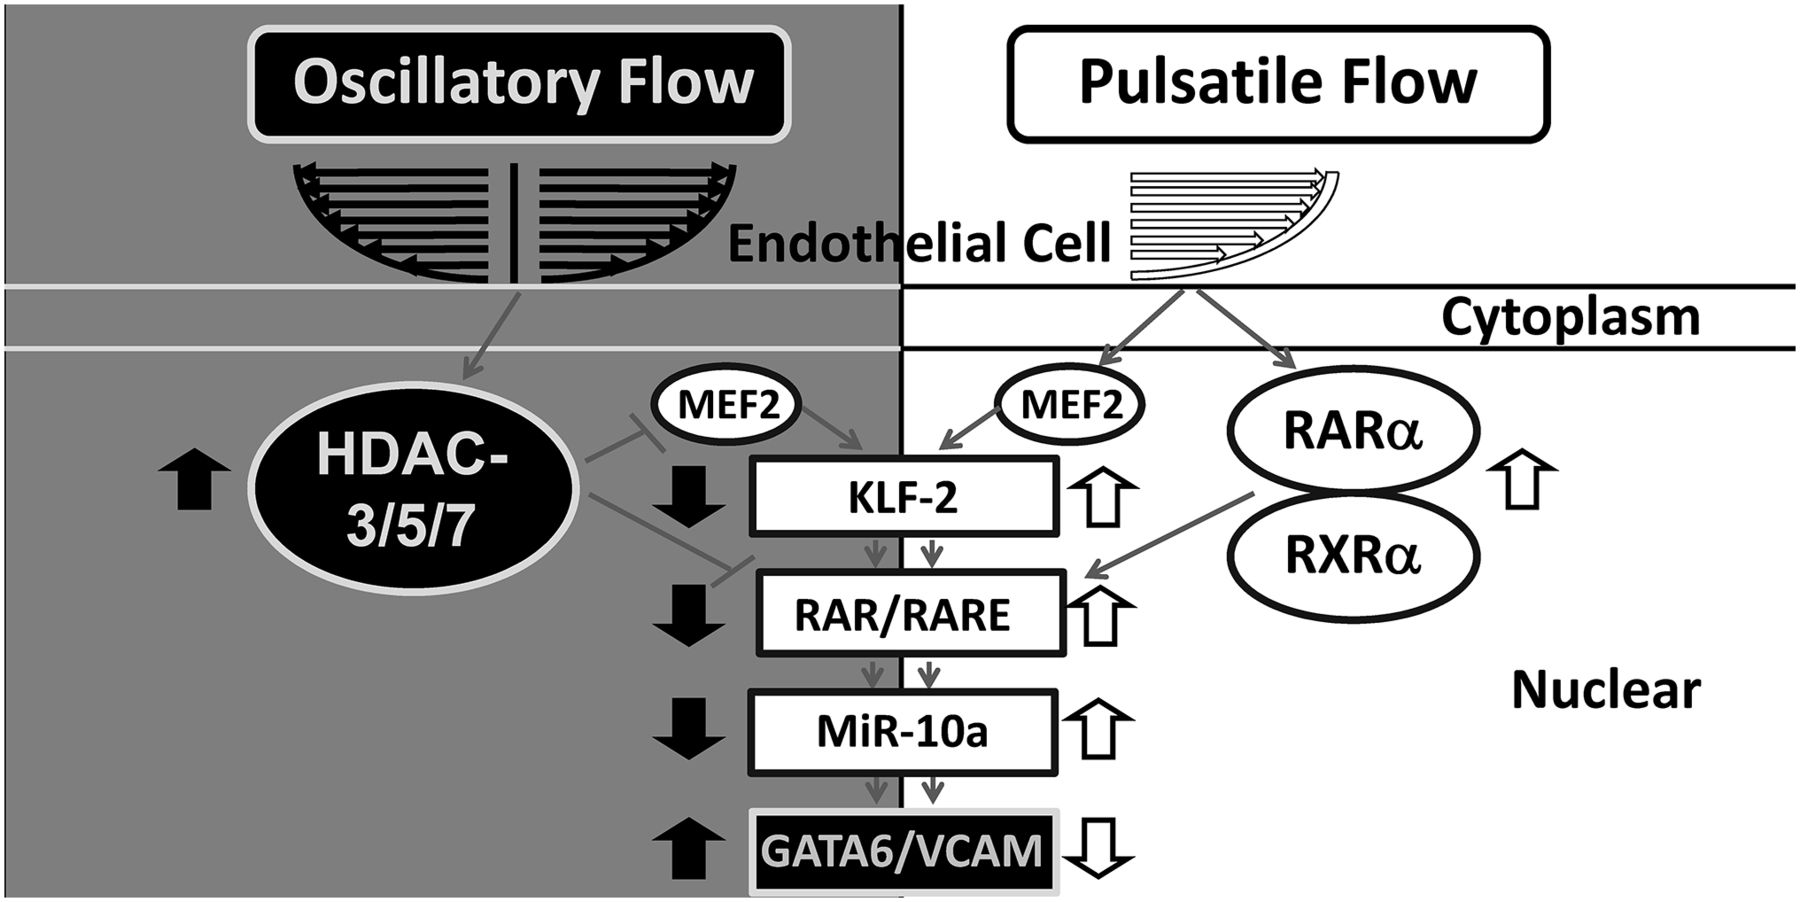
\includegraphics[width=.7\textwidth]{figures/mir10-circuit}
\caption[HDAC7/RARA/miR-10a Circuit.]{\textbf{Schematic diagram of the roles of hormone receptors and HDACs in modulating miR-10a expression and hence proatherogenic and antiatherogenic signaling in EC in response to different flow conditions.} Boxes with black and white shading represent proatherogenic and atheroprotective molecules, respectively. Image and caption from Lee \emph{et al.}\cite{Lee2017}
\label{fig:mir10-circuit}}
\end{figure}

\subsection{RNA Sequencing} \label{sec:discussion:rna-seq}
By 2020, \ac{seq} has by and large outgrown the teething troubles of its initial technological phase. However, the method itself brings with it inherent, largely mathematical problems. A lack of reproducibility was a great concern in the initial periods of RNA-seq, but the reproducibility of cholinergic cell culture (Section \ref{sec:cellculture:sequencing}) as well as the validations performed on small RNA during the studies of stroke patient blood (data not shown in this dissertation, but in the associated publication\cite{Winek2020}) show an agreeable reliability of the method in our hands.

Unrelatedly, the multiple testing problem still remains a pertinent issue of modern molecular biology. It is now more impressive to find a negative result in one of these analyses (e.g., no differential expression in a reasonably powered sequencing experiment) than it is to find actual differences. The question of where to place the threshold of significance, or whether to use such a threshold at all, is still a matter of very lively debate among scientists of many disciplines; additionally, consensus thresholds vary between fields or even between different kinds of assay. This dissertation, in general, follows the philosophy of balance between limiting false positives (by monitoring false discovery rate and utilising cross-experimental comparison) and identifying »real« changes (by monitoring adequate powering and effect sizes). In the limited area of RNA-seq, this is still manageable, because standard approaches in the form of multiple correction for differential expression analysis (e.g. in DESeq2,\cite{Love2014} which essentially uses Benjamini-Hochberg correction) and power analysis packages (I used R/powsimR\cite{Vieth2017}) already exist; in the extended graph-based network analyses, the matter is more complicated (see below in Section \ref{sec:discussion:network-statistics}).

For sequencing, particularly of small RNA, there remain open questions about the nature of detection. For instance, the alignment from raw sequencing reads of the two different smRNA species surveyed in Chapter 4 is handled by two separate software solutions, each tailored exactly to the biological nature of the respective smRNA species. I used miRExpress, version 2,\cite{Wang2009} to align miRNA sequences, and MINTmap\cite{Loher2017} for the tRNA fragments (more specifically, only the fragments »exclusive to the tRNA space«). Procedurally, there is no argument or consensus against analysing these two species separately, and unifying results afterwards. The main effect of concatenation of the two count tables for joint analysis in DESeq2 differential expression analysis is a loss in sensitivity, because multiple testing has to be corrected in relation to the number of unique analytes. However, since the hypotheses assumed before analysis included modes of cooperation between the two distinct species, I decided to test them together rather than apart from each other. The inspection of MA plots (see e.g. Figure \ref{fig:apeglm-comp-la2d4}), effect size distribution, and the comparison to separate analyses for both species all indicated the joint approach to be feasible. The loss in specificity was mild in miRNAs, joint analysis reproduced 98.4\% of detected and 83\% of differentially expressed miRNAs (FDR < 0.05), and 98.3\% of differentially expressed miRNAs with high effect size (absolute \ac{lfc} > 1.4). For tRFs, the loss was greater; joint analysis reproduced 96.1\% of detected, but only 20.5\% of differentially expressed tRFs. This can be explained by a high number of very lowly expressed tRFs compared to miRNAs: tRFs with high differential expression effect size (\ac{lfc} > 1.4) were reproduced at 52.1\%; and reproduction in the top 5 percentile by count-change was 92.3\%. Notably, this 95th percentile count-change cutoff value is at an absolute count-change of 28.5, meaning the loss of differentially expressed tRFs compared to separate analysis happened in the very low expression range, which is more desirable than it is a problem. An alternative solution would have been the truncation of low-count analytes before differential expression analysis; however, the threshold for such a step is always arbitrary, and thus truncation is no longer recommended.\cite{Zhu2019}

\subsection{Statistical Analyses of Network Interactions} \label{sec:discussion:network-statistics}
There is much less consensus when it comes to statistical interpretation of network analyses. This may in part be a result of network analyses being relatively uncommon compared to, for instance, sequencing experiments, and thus a lack of community consensus on how to approach certain problems. Often, a »network analysis« is a very confined, ultimate visualisation of the impact of one or few miRNAs with several genes that seem pertinent to the publication (for an example see Figure \ref{example-network}). Thus, there is often no need to characterise the statistical relevance of the shown relationships, as they serve as a visualisation of hypotheses, or an illustration of a proposed pathway. In contrast, most network analyses presented in this dissertation are intermediary steps, the results of which are supposed to aid in identification of pertinent factors in the molecular interactions studied. As a result, there is a need to measure the relevance of each component of the network, as well as the validity of its message as a whole. Those can be approached in different ways, as is described in the following.

\begin{figure}
\centering
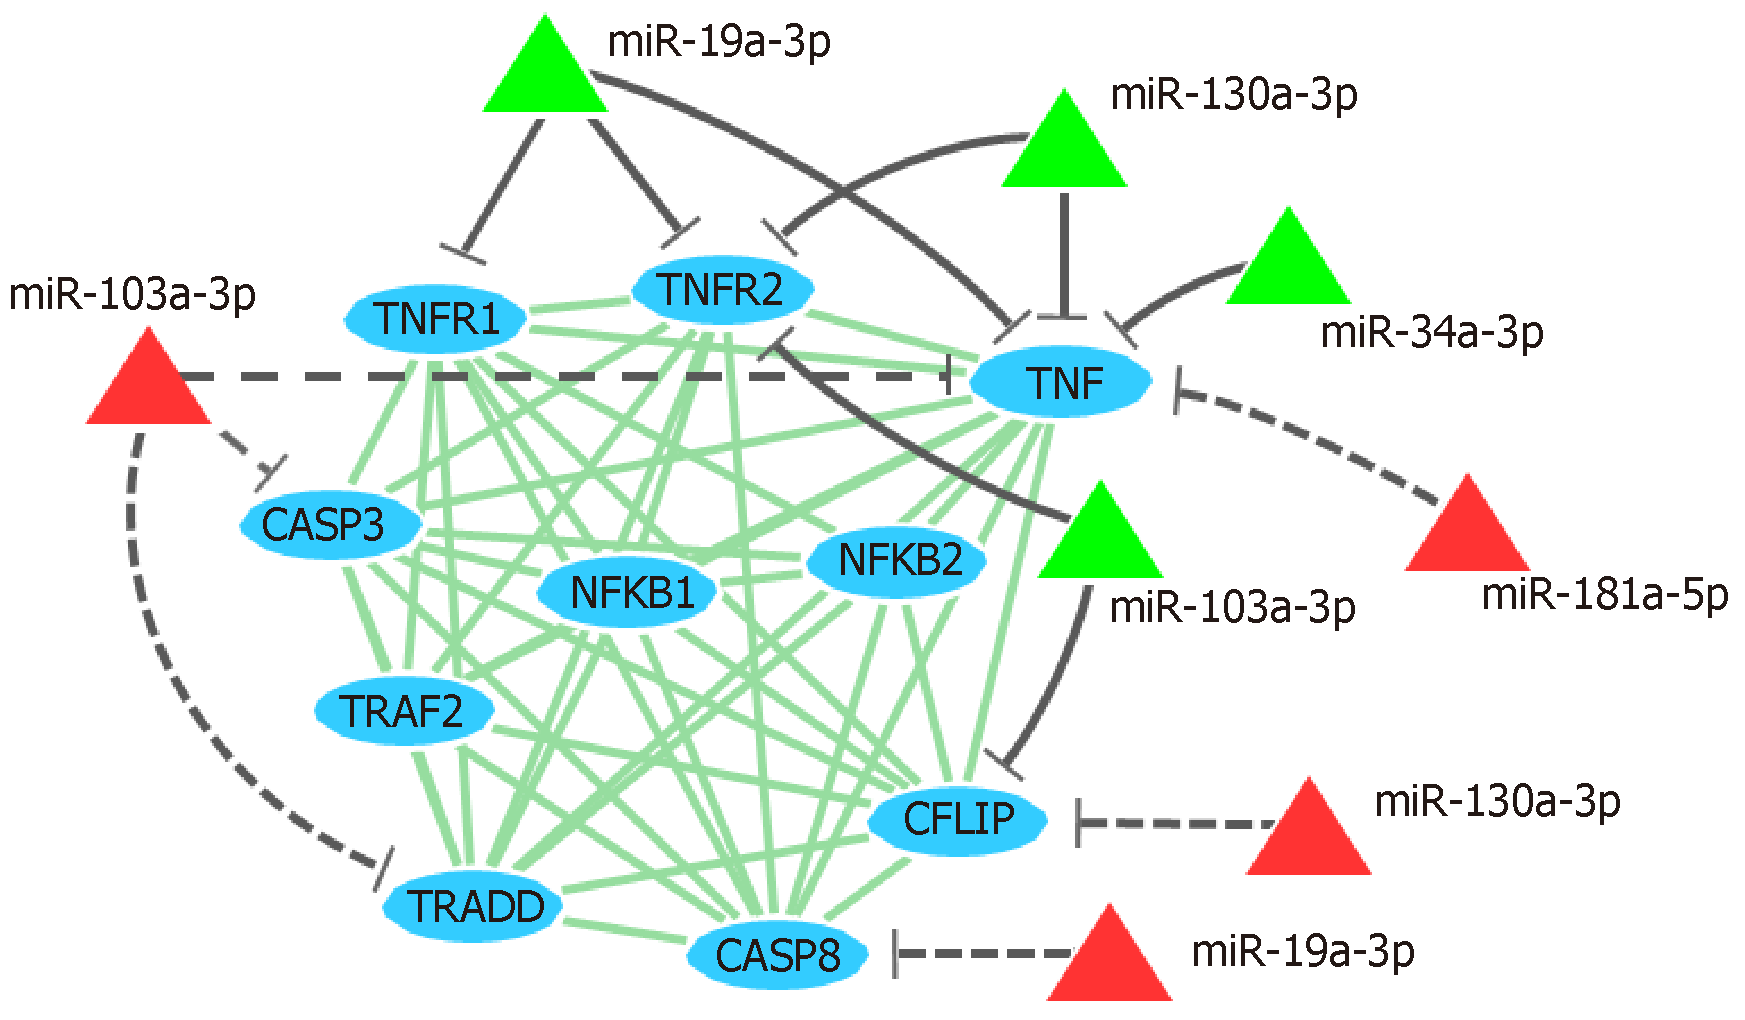
\includegraphics[width=.6\textwidth]{figures/example-network}
\caption[miRNA-Interaction Network Example.]{\textbf{Interaction network showing miRNAs and their predicted and validated targets.} The protein interaction network (light gray lines) shows the interaction between proteins (ellipses) encoded by tumor necrosis factor-$\upalpha$ pathway genes. Green triangles and solid gray lines represent miRNAs and validated target genes, respectively; red triangles and dotted gray lines represent predicted relationship between miRNA and target genes, respectively. TNF: Tumor necrosis factor. Image and caption from Rossi \emph{et al.}\cite{Rossi2019}
\label{fig:example-network}}
\end{figure}

The validity of single network components is subject to various pre-existing properties. To make this discussion more tangible, I will give an example of the most common single component in my analyses: a miRNA$\to$gene interaction. A first measure of its validity can be the existence of a validation experiment of this interaction. This is reflected in the scoring inside the database. The limitations as discussed in Section \ref{sec:discussion:mirneo}, e.g. in regard to tissue specificity, still apply. Below this highest level of stringency are the predicted interactions. As has been discussed previously by others, miRNA$\to$gene relationship predictions are best seen in comparison to other models, and most valuable predictions are the ones that several prediction algorithms agree upon, particularly if these algorithms are based on modelling different aspects of miRNA$\to$gene binding.\cite{Witkos2011} For this reason, I implemented the largest collection of algorithms I could find at the time (miRWalk 2.0\cite{Dweep2015}), supplemented by other sources as they became available, and also statistically evaluated the performance of all included algorithms to select a suitable subset for the summation of scores (Section \ref{sec:database:mirna}). These steps were undertaken to minimise the risk of bias by using as many sources as possible, while still retaining an amount of flexibility in analysis. For instance, if the resulting gene network was too large for sensible analysis, its size could be easily decreased by elevation of the score threshold, thus making the analysis more stringent.

The scoring threshold as used for miRNA interactions is not available for tRFs, because there are no prediction datasets available yet. The prediction was performed in-house on miRNA-like seeds of each detected differentially expressed tRF, which brings two important limitations: it assumes a miRNA-like functionality of tRFs, disregarding other interaction principles that have been found (see Section \ref{sec:intro:trfs}); and it limits the prediction sources to one, TargetScan.\cite{Friedman2009} TargetScan was selected for its approach of measuring evolutionary conservation of putative target sites, a measure that is very valuable in the case of tRFs, because we know little about any other parameters that could be relevant for the targeting. Since tRNAs and their fragments have been part of mammalian cells for a long time, evolutionary conservation of target sites in the genetically flexible 3' UTRs is a significant measure of functionality.\cite{Agarwal2015} Thus, for tRFs, the aggregation score of multiple algorithms was substituted with the conservation score generated by branch length (BL) and probability of conserved targeting (P$_{CT}$).\cite{Agarwal2015}

However, these cautionary steps still cannot preclude any and all possible biases that may be inherent to prediction models, and thus, statistical analyses on the basis of this general procedure are desirable. The simplest, most practical, although computationally intensive solution to inherent database biases is permutation (see Section \ref{sec:database:permutation}). Briefly, a null distribution of the measured parameter (e.g., miRNA$\to$gene interaction score) is generated by iterative analysis of randomly permuted datasets of the same size as the »real« dataset to be tested. The location of the »real« score inside this null distribution then gives the »extremity« of that real result, and thus the likelihood of the result being as extreme by chance, which equals \acf{fdr}. However, this approach requires a defined set of analytes that present with a measurable attribute (e.g., multiple miRNAs targeting one gene, or a defined set of target genes for any one miRNA). An additional measure to ensure robustness of this approach is the iteration across a range of parameters, for instance, a sliding score cutoff. Results staying »significant« across a range of different cutoffs may be an indication of their robustness. However, for each level of iterations added, computation time also increases. Since permutation approaches usually require tens to hundreds of thousands of iterations, the computational requirements can be considerable.

The advantage of permutations, as opposed to the disadvantage of having to test a set of multiple entries, is its scalability. Thus, permutations can also be used to assess the validity of the entire network, for instance by random permutation of case-control status (applicable in patient scenarios, as in Chapter 4), or of another attribute (such as sex, as in Chapter 3).

\subsection{Cholinergic Cellular Models: LA-N-2 and LA-N-5}
The decision to use a human cellular model of cholinergic neuronal cells was driven by two main factors: I) \emph{In vivo} experimentation, i.e., animal-based research, is not reliable as a model of complex human psychiatric diseases.\cite{} II) Particular to RNA-based mechanisms, the difference between rodent and human genes is enormous, for instance in 3' UTRs that are not subject to the same evolutionary pressure as coding regions, which leads to low transferability of the application of hypothetical therapeutic oligonucleotides.\cite{} Furthermore, so-called »3D cell cultures« or co-cultures of human cells of different types (e.g., neurons with astrocytes) are still not as developed as is necessary for stable experimentation, particularly in the case of cholinergic systems;\cite{} thus, we opted for mono-culture of neuronal cell lines. Even in traditionally cholinergic research, the number of human neuronal models representative of actual cholinergic neurons is very low; the popular cell line SH-SY5Y had to be excluded after in-depth experimentation because it fails to express sensible amounts of the main cholinergic marker \emph{CHAT} and the vesicular transporter \emph{SLC18A3} even upon differentiation (own results, unpublished).

LA-N cells were the logical alternative in the search for an adequate cholinergic model, although their maintenance is not as straightforward as that of many of the work-horses of human cell culture. The main argument for their selection was their natural expression of \emph{CHAT} and \emph{SLC18A3} as well as an impressive induction of these genes via stimulation by neurokines. This expression of \emph{CHAT} is a pivotal factor in the studies of cholinergic neurons, because there is much confusion about what constitutes a cholinergic cell in the CNS, and about the properties of the different cholinergic populations in the different brain regions. By definition, cholinergic neurons must be able to synthesise ACh (\emph{CHAT}) and release it through vesicles (\emph{SLC18A3}). Additionally, the high affinity choline uptake mediated by the SLC5A7 transporter is highly correlated with these two central markers in the nervous system (own results, Figure \ref{fig:chat-hacu-corr}, Yuliani \emph{et al.}\cite{Yuliani2020}). Other defining properties of cholinergic neurons are more optional (for instance, the defining property of basal forebrain cholinergic projection neurons to receive the retrograde NGF signal via \emph{NTRK1}). An additional benefit was the availability of LA-N cells of both sexes, which aided in studying sex differences in Lobentanzer \emph{et al.}\cite{Lobentanzer2019a}

\begin{figure}
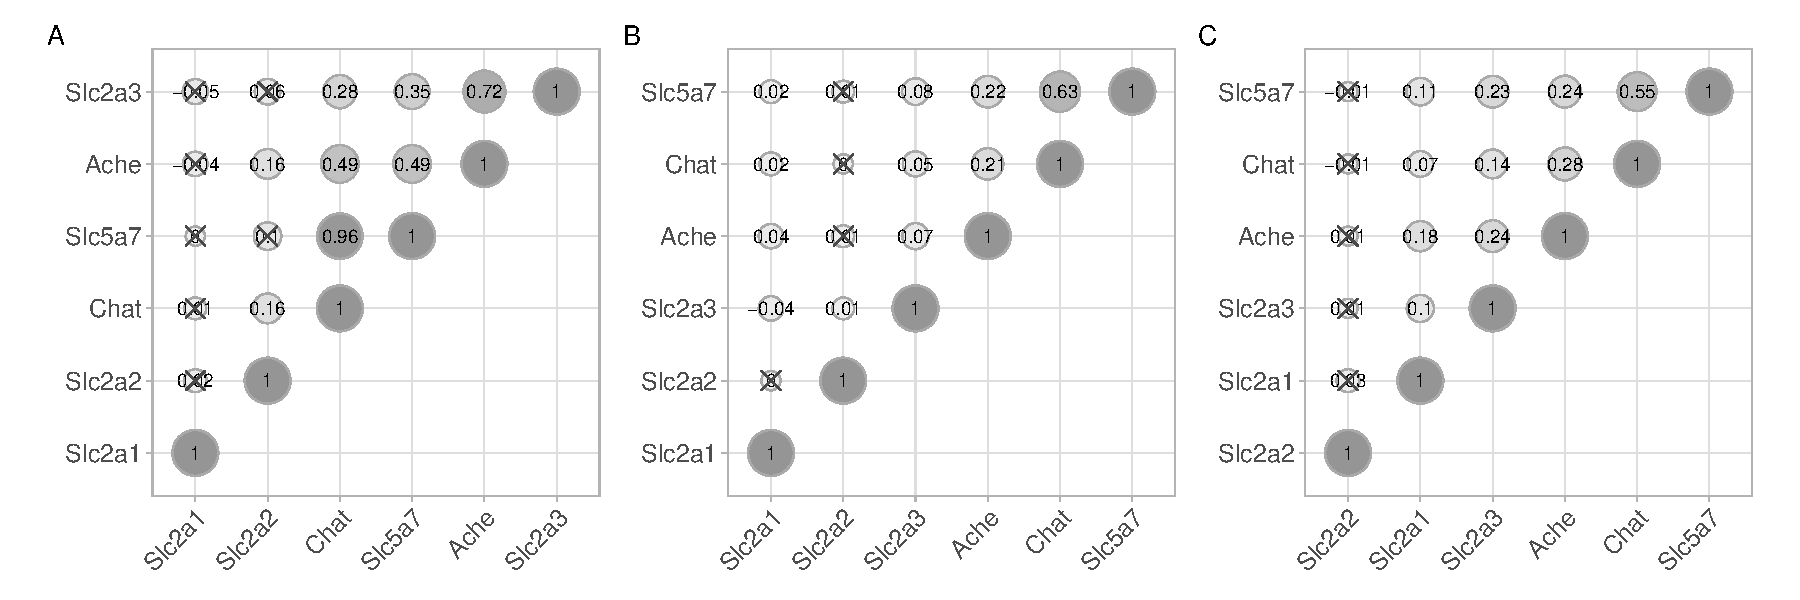
\includegraphics[width=\textwidth]{figures/chat-hacu-corr}
\caption[Correlation between CHAT and HACU in Nervous Cells.]{\textbf{Correlation between CHAT and HACU in Nervous Cells.} Size and depth of colour of circles denote strength of correlation (Pearson’s product-moment correlation coefficient, PPMCC), numbers denote PPMCC (range: -1 to 1). Non-significant correlation coefficients (p > 0.05) are crossed out. Rows and columns are ordered by hierarchical clustering, representing similarity of PPMCC values (Euclidian distance). (A) Correlation of transcripts in all tissues (cell-type-level) of the murine nervous system. (B) Correlation in all neurons (single-cell-level) of the murine nervous system. (C) Correlation in cholinergic neurons (single-cell-level) as determined by expression of the vesicular ACh-transporter, SLC18A3. Modified from Yuliani \emph{et al.}\cite{Yuliani2020}
\label{fig:chat-hacu-corr}}
\end{figure}

The decision for a mono-culture of immortalised human neuronal cells naturally introduced limitations common to all similar models: the cells are derived from tumour cells and do not resemble a physiological cell any more, otherwise they would not have lost senescence. All biological implications derived from these models have to be interpreted based on this central limitation. However, interpretation is based on the assumption that basic molecular processes, such as the control of mRNA by miRNAs, are still intact. Additionally, the cell communities generated \emph{in vitro} that are the basis of bulk sequencing analyses are very homogeneous, more so than any tissue derived from a living multi-cellular organism. While this enables bulk sequencing without »dilution« by supporting CNS-derived cells, as would be the case in patient brain region bulk sequencing, it also introduces a »non-natural« homogeneity in the RNA derived from the lysis of these cells and therefore harbours the danger of exacerbated sensitivity in differential expression. This may lead to the false positive identification of differentially expressed smRNAs, particularly those with a low base expression or small changes. However, controlling of effect sizes (e.g., a cutoff for absolute \acl{lfc}, or analysis of count-change) is well suited to prevent many irrelevant false positives.

\subsection{Stroke Patient Blood Samples} \label{sec:discussion:stroke-blood}
The main limitations in the sequencing of post-stroke patient blood are the lack in cell type specificity of RNA generation and the composition of the patient collective, which resulted in exclusion of females for balancing reasons and thus contains only male patients. Additionally, the controls by principle have to be external, since stroke is an unexpected event and thus there is virtually no possibility of attaining a blood samples of patients pre-stroke except in very specific clinical conditions. As a result, control samples are healthy volunteers, that have to be matched in a manner that reproduces the patient collective as closely as possible, which often cannot be more specific than matching for sex and age. Strictly speaking, the results of analyses based on the differential expression profile can only be applied to male patients. However, the tissue-specific analyses performed on small RNAs as well as on transcription factor interactions are based on large data collections representative of many male and female volunteers, and thus the CD14$^+$-related analyses, such as the \acf{ffl} analysis in Section \ref{sec:stroke:ffl-cd14}, can in large parts be applied to both sexes.

Section \ref{sec:stroke:celltypes} exclusively deals with the shortcomings of sequencing whole blood instead of isolated cellular components. Whether this method of extrapolation serves the purpose of explaining the roles of the tissues involved in smRNA stroke response remains to be clarified. However, translational approaches such as the one presented in Section \ref{sec:stroke:celltypes} can also aid in studying the transferability of whole blood results (which may be more common in the clinical setting) to tissue-specific analyses, which often require complex and costly purification steps in acquiring the isolated cell populations.

\subsection{Gene Ontology Analyses} \label{sec:discussion:go}
Some of the approaches to dimensionality reduction presented here rely heavily on the analysis of enrichment of genes in ontological categories of biological processes. The primary purpose of using GO enrichment as a tool is to deal with the reality of not being able to know all functions of any given gene. Strictly speaking, here also apply the same limitations as to other datasets of curated information: the quality of results depends on the quality of annotation in the raw ontology collection. For some lesser known proteins, these annotations may well be far from complete, and thus result in presentation bias towards the interpreting scientist. Similarly, by interpreting the list of ontological terms yielded by an analysis, terms may be selected or discarded based on their perceived relevance to the topic of study; inadequate knowledge about all participating processes may lead to the dismissal of relevant terms, constituting confirmation bias. To try and avoid large amounts of this form of confirmation bias, GO terms were presented in comprehensive form or as curated form of all available data as much as possible (see for instance Figure \ref{fig:mir-de-fam-go}\,B and Section \ref{sec:stroke:ffl-cd14}). Additionally, the visual display of GO terms as a t-SNE projection, where distance is based on the amount of shared genes between the terms (using R/gsoap\cite{Tokar2020}), can aid in identifying the underlying categories of processes, and their relationships to one another. This is aided by the weighing functionality of R/topGO analysis,\cite{Alexa2006} whereby less specific parent GO terms are dismissed in favour of the more specific child nodes in the DAG graph (see also Sections \ref{sec:database:gsea} and \ref{sec:cellculture:topgo}).

An intriguing possibility is the transfer of ontology analyses of smRNA-targeted protein-coding transcripts to facilitate an understanding of the biological processes controlled by the smRNA interference. The approach is still underdeveloped in several regards: I) The weighing of smRNA$\to$gene relationships has a large influence on the outcome, making iteration and testing of robustness indispensable. II) The resolution of annotation is much coarser than in direct gene annotation. Due to the many-to-many nature of the miRNA interactome, functional implications for any one miRNA strongly intersect with other, similar miRNAs. This is the main reason for the analysis of families instead of single miRNAs in Section \ref{sec:cellculture:topgo}. In summary, while the derivation of function of miRNAs from their targeted genes is tempting in the light of a complete lack of direct functional annotation for miRNAs, this projection approach will have to be developed and validated before it can be routinely applied.

\subsection{Feedforward Loop Analyses} \label{sec:discussion:ffl}
Feedforward loop analysis brings together most of the issues discussed above. I) It is based on the aggregation of several types of molecular targeting relationships and thus is subject to their individual limitations. II) It is applied to the results of differential expression in stroke patient blood, and thus is also influenced by sequencing-related issues. And III) The modules yielded by FFL stratification are then scrutinised with the help of GO analysis to find gene collectives relevant to stroke.

Regarding I); the results of concatenation of these individual relationship types are unknown and difficult to measure. Every kind of influence on the validity of results is imaginable: the insecurities from each individual method might be additive, or even super-additive, making the end result more unreliable in consequence. Alternatively, the processes being firmly rooted in the biological reality of the cell might also have a corrective function on the end result, effectively acting as a filter that removes »illogical« circuits from the output, thus increasing its validity. There is no measure for answering this question as of now. However, the circuits and their ontological associations gathered in Chapter 4 make sense from a biological perspective, and, maybe more importantly, they make more biological sense than an observation of only differentially expressed genes, or only of smRNAs. In short, although the evidence is circumstantial, the message gained from FFL analysis may be larger than the sum of its parts. A more detailed discussion of the individual findings is held in the individual module descriptions of Section \ref{sec:stroke:ffl-cd14} and Section \ref{sec:stroke:resolution}. The substantiation of FFL analyses and their biological meaning is an important topic for further research.

Regarding II); sequencing-related issues need to be primarily controlled in the process of differential expression analysis. During feedforward loop analysis, results from differential expression are fixed, and thus cannot cause much confounding if they are used in a descriptive way, as is the case in my analyses. Should they be used beyond that, for instance, to weigh targeting relationships by the differential expression of their participating factors, more care has to be taken that the model applied makes sense. Although the approach is feasible in principle, the practical application in FFL analysis is not trivial. Generally, it makes sense to compare the expression levels of smRNAs and their target genes, for two main reasons: 

One, any interaction probably only has practical relevance in the cell if the expression levels (or rather, the change in expression), is on the same scale for both smRNA and mRNA. Of note, the count-change measure introduced in Lobentanzer \emph{et al.}\cite{Lobentanzer2019a} is much more suited to this assessment than the commonly used \ac{lfc}, because the latter does not relate to expression levels at all. However, until the sequencing of small and large RNAs can be routinely done in the same experiment (i.e., on the same microfluidic chip), the comparison of base mean expression (or count-change) between small and large RNA will always be very approximate, because it is dependent on sequencing depth of the individual experiment. 

And two, considering miRNA-like interactions, those interactions will be particularly interesting where the smRNA is regulated inversely to the target mRNA. However, this concerns only the theoretical interaction of two isolated partners, whereas the smRNA$\to$gene interactions in live cells are layered and only the strongest single relationships will have a chance of prevailing against the regulatory »chaos« that is an actual cell. This alone precludes actual analysis of differential expression influence on smRNA targeting (apart from complex mathematical models which remain to be established), without even considering the third interaction partner, transcription factors. Those introduce another element of uncertainty: although we know more about their tissue specific activities through efforts such as Marbach \emph{et al.}\cite{Marbach2016}, we do not specifically know which transcription factor acts on a promoter or repressor towards which genes in which tissues. Mathematical structural models able to predict these interactions in a cellular, whole-genome context are desirable, but not yet a reality.

Regarding III); the main criticism of proceeding from comprehensive FFLs through modularisation to GO analysis is the arbitrary nature of network modularisation. Modularisation itself is a purely mathematical process of describing the interconnectedness of nodes in the network, implemented by Blondel \emph{et al.} (»Fast unfolding of communities in large networks«).\cite{Blondel2008} The choice of resolution that yielded five communities in my analysis thus was largely arbitrary, selected in a way that correlated module identity with the visual clusters created by force-directed organisation of the FFL network. However, since the main purpose of modularisation is a reduction in dimensionality that facilitates human understanding, every possible resolution that results in a manageable number of modules may be seen as »reasonable«. A standardisation of these procedures is nevertheless desirable and will be subject of further studies.

%\newpage

%!TEX root = ../dissertation.tex
\section[A Mechanistic Perspective of Transcriptional Interactions]{A Mechanistic Perspective of \\Transcriptional Interactions}

This dissertation is aimed at elucidating epi-transcriptional processes surrounding the expression of cholinergic genes. To this end, a framework was developed to assess interactions between players on the field of RNA-related processes in mammalian cells. This framework was then applied to state-of-the-art measurements of RNA levels, i.e., RNA-sequencing. In the following paragraphs, an assessment will be held on the outcomes of my efforts in clarifying »Small RNA Dynamics in Cholinergic Systems«.

\subsection{Analysis of Small RNA Dynamics via RNA-sequencing \\and Bioinformatics}
Small RNAs and the mechanisms by which they control the expression of coding genes have fascinated researchers since their discovery around the turn of the millennium. Much of the pioneering work has been done on miRNAs, but with tRFs, a new class of regulatory small RNA is increasingly being investigated in physiological and pathological contexts. During the current, early phase of small RNA studies, research has often assumed a limited perspective; many publications study interaction between few partners, in most cases reducing focus to one miRNA and one targeted gene. However, during the initial phase of my work on transcriptional interactions, it quickly became apparent that an integrative perspective is crucial. First and foremost, this involves information on the coding genes that are the supposed targets of small RNA intervention, but also the workings of transcription factors, which shape the phenotype of the cell, and, relatedly, tissue specificity of all of the aforementioned processes.

As such, a comprehensive integrative model of smRNA interactions did not exist when I started to work on this dissertation. More recently, there have been developments of integrative databases which model miRNA$\to$gene interaction, one of them also including tissue specificity and transcription factors. The most extensive efforts in my view are mirDIP, miRWalk 3.0, and miRNet (causing the name change of my own database). Thus, they will be briefly reviewed and compared to my own work in the following.

mirDIP 4.1\cite{Tokar2018} and miRWalk 3.0\cite{Sticht2018} are similar in their focus on miRNA$\to$gene interactions. To this end, both collected and integrated third-party data into their database. Both offer public access through a browser-based interface and database downloads. In addition, mirDIP offers integration into development environments via Java, R, and Python APIs. The main difference between the two is their data aggregation approach. While the mirDIP team collected all resources available (75 different sources\cite{Tokar2018}), the miRWalk developers reduced their source count between versions 2.0 and 3.0, from 12 sources to 4.\cite{Sticht2018} Instead of combinatorial power, the authors of miRWalk 3.0 rely on a single algorithm as core principle of miRNA$\to$gene targeting, TarPmiR.\cite{Ding2016} Briefly, TarPmiR utilises machine learning (random forest) to identify miRNA binding sites by characteristics learned from photoactivatable-ribonucleoside-enhanced crosslinking and immunoprecipitation (PAR-CLIP) sequencing results. A comparison to other prediction algorithms indicated superior performance in the authors' hands.\cite{Ding2016} However, it also shows how incomplete these approaches still are: the average recall of TarPmiR in the initial publication was 0.543, and the precision was merely 0.181 (or 0.191, the numbers in the manuscript conflict), indicating a high number of false positives. In light of these numbers, reliance on any one algorithm still remains statistically inferior to the combination of predictions based on different modelling techniques.\cite{Witkos2011} In light of the reliability of prediction algorithms, which ranges from very low to medium at best, stringent assessment of statistical properties of these data collections is necessary. However, the authors of miRWalk 3.0 have not statistically evaluated the performance of their database in the most recent publication.\cite{Sticht2018}

At the other extreme, mirDIP 4.1 includes 30 publicly available sources, selected from a review of 75 sources, to yield a total amount of 150 million targeting predictions.\cite{Tokar2018} Of note, due to performance issues (space requirements and query times), the database only supports miRNA:gene interactions, without additional information such as mRNA binding site, and does not work with gene identifiers other than HUGO symbol (which may be ambiguous). For integration of all third-party datasets, the authors normalised confidence levels of predictions inside each dataset to yield a score between 0 and 1, and then ranked each prediction dataset based on a benchmarking procedure (using experimentally validated interactions). These ranks were then used to calculate the confidence of miRNA$\to$gene relationships via an integrative scoring, similar to the score in \emph{miRNeo}, but with the addition of a weight for each prediction dataset. The addition of a weight may be beneficial the more source datasets are used, to differentiate between different qualities of source material. What I did by excluding the two poor performance datasets (Section \ref{sec:database:mirna}) equals a simplified weighing procedure (with score of 1 for included datasets and 0 for dropped). A comparison of \emph{miRNeo} accuracy compared to the mirDIP 4.1 data using the benchmarking data will be interesting, but has not been performed yet. Once the mirDIP data is integrated in \emph{miRNeo}, the benefit of the weighing procedure can be evaluated.

\emph{miRNeo} is not designed to compete with these types of database; on the contrary, \emph{miRNeo} relies on a combination of publicly available datasets to enable accurate prediction\cite{Witkos2011} and to be able to derive test statistics from comparison of different source materials. Rather, \emph{miRNeo} is designed to be efficient in managing complex computations on RNA-based interactions so as to enable the study of complex relationships and biological mechanisms such as feedforward loops.

As such, miRNet\cite{Fan2016} is closest in functionality to \emph{miRNeo}, as it provides interaction data on transcription factors as well. Very recently, it seems to have been updated to version 2.0, which allows study of transcription factors and feedforward loops, but there has been no publication detailing the results as of yet (April 2020). Its main »advantage« (see below) over \emph{miRNeo} for users is that it provides an easy-to-use web-based interface for analyses; its main downside is that it practically includes only two main miRNA targeting sources, TarBase and miRecords. miRNA:TF data were collected from a dedicated source, TransmiR, which includes only manually curated interactions, and thus likely underestimates the true interactions by orders of magnitude. Additionally, the new version of miRNet seems to diverge significantly from the original description,\cite{Fan2016} and the only way of evaluating the database is by the very limited »About«-section on the webpage, which unfortunately features several inconsistencies. For instance, the authors state that »miRNA to TF interaction data were collected from TransmiR 2.0«, however, TransmiR is a TF$\to$miRNA database, which is critically and fundamentally different in its implications. In addition, a curated database such as TransmiR cannot currently be designated comprehensive, by their own description it includes »2,852 TF-miRNA regulations from 1,045 publications«, and very limited tissue-specific information. However, in the miRNet web application, tissues can be selected for TF interactions, regardless of target type. How that is possible is not explained. In summary, while the idea behind miRNet may be similar to \emph{miRNeo}, function and performance cannot currently be assessed without additional information on what exactly miRNet does, and what data it is based on. It may even be dangerous to present researchers with such an easily accessible tool, a »black box«, which from the input of only a few gene names generates complex analyses without requiring any understanding from the researcher performing the analyses. Maybe even more questionable is the lack of transparency as to how the results are generated. Taken together, it harbours the danger of generating a large amount of false results, and consequently, a number of irreproducible research findings.

In summary, \emph{miRNeo} as an integrative approach to small RNA dynamics is a valuable addition to the repertoire of the study of transcriptional interactions. It collects several resources for targeting of genes by small RNAs, which have been statistically evaluated as to their performance; it integrates this targeting data with tissue-specific TF$\to$gene targeting information from 394 human tissues, based on the \mbox{FANTOM5} dataset; and it provides, through its graph-based infrastructure, high computational performance for the assessment of complex relationships in RNA interaction. From these vantage points, it is the most complete integrative transcriptional interaction database to date. Its main limitation in this context is the limited availability due to the lack of a web-interface or public R package, and the high entry-level of knowledge it requires for usage.

\subsection{The Cholinergic/Neurokine Interface}
Multiple lines of orthogonal evidence confirm the significance of neurokines for cholinergic processes, and imply a cooperation between cholinergic and neurokine systems in health as well as in disease. Earliest descriptions of neurokines, in the late 1980s, have tied them to cholinergic differentiation, which was the reason for adopting the LA-N cell models for experimental work in this dissertation.\cite{} The bioinformatic analyses of these experiments identified two miRNA families, mir-10 and mir-199, to inhabit a pivotal role in interfacing between cholinergic and neurokine genes, and transcriptomic analyses of single cell data from murine and human CNS demonstrate a co-expression of cholinergic markers and neurokine receptors.\cite{Lobentanzer2019a} Thus, an assessment of cholinergic neuron functionality, be it in health or in neurological disease, has to take into account these para- and endocrine influences, particularly from the neurokine and neurotrophic factor families. 

More generally, it is very likely that most neuroscientific endeavours would benefit from integrating other aspects of life-science, in particular, endocrinology and immunology. As recent literature shows, many classifications of diseases originally thought neurologic are currently being revised, often resulting in inclusion of immunological aspects; first and foremost, the term »neuroinflammation« has seen a rise in popularity by 806\% in the last decade (PubMed search results of publications between 1900 and 2010: 2414, between 2010 and 2020: 19465, Figure \ref{fig:pubmed-neuro}). Consequently, the scientific community has much to gain from cooperation between the neurologic and immunologic branches of research.

\begin{figure}
\centering
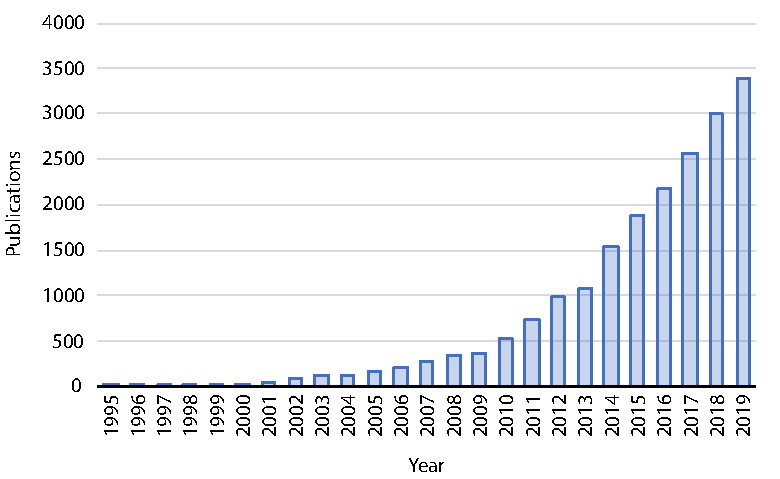
\includegraphics[width=0.7\textwidth]{figures/pubmed-neuro}
\caption[Number of Publications on Neuroinflammation by Year.]{\textbf{Number of Publications on Neuroinflammation by Year.} Data were downloaded from https://www.ncbi.nlm.nih.gov/pubmed on the first of April 2020.
\label{fig:pubmed-neuro}}
\end{figure}

Importantly, the interaction between neurokine and cholinergic systems is not unidirectional; both systems control manifold properties of the mammalian body, and thus, communication between the two systems takes place in various ways, cell types, and organs of the body. Arguably, the most immediate form of this communication is the elicitation of cholinergic properties in neuronal cells by neurokine signals. It has been shown by myself and others that isolated neuronal cells express more \acf{chat} and \acf{slc} upon neurokine stimulation,\cite{} and stimulation by \acf{lif} results in catechol"-amin"-ergic$\to$cholin"-ergic transformation of sympathetic neurons \emph{in vivo}.\cite{} In theory, this type of interaction between neurokine and cholinergic systems requires only one type of cell (if the neuron in question were able to synthesise and release a neurokine); however, \emph{in vivo}, it likely involves at least two types of cells: the neuron receptive of the neurokine signal, and a regulatory cell which releases the neurokine. While the regulatory cell types releasing IL-6, the most studied neurokine by far, are already well described, the cellular sources of the other, lesser-studied neurokines are still enigmatic, particularly in the CNS. Similarly, the differences in effect on the stimulated cells by the different neurokines, which in all likelihood are rather subtle, have not been studied as of yet. By the rather unique combination of soluble and membrane-bound receptors, which cooperate in a fashion unique to each individual member of the gp130 family, neurokines present a tremendously complex regulatory mechanism.

Conversely, cholinergic systems can influence neurokines, however, this side of the interaction is much less clear and subject to considerable controversy. While the definition of »cholinergic« is relatively simple in the transcriptional context, a clear definition of neurokine tissues is all but impossible. A cholinergic neuron by definition is characterised by its expression of CHAT and SLC18A3, without which it would not be able to transmit a cholinergic signal; in the case of non-neuronal cholinergic systems, it is admittedly more complex. In neurokine systems, however, most cell types that may be considered as candidates fulfil a wide range of functions, using multiple and diverse messenger molecules; mainly, this involves tissues of the immune system. As such, the »target cell« of cholinergic$\to$neurokine interaction may be different depending on the context, which complicates the analysis of clinical and experimental data. The most prominent instance of cholin"-ergic$\to$neuro"-kine interaction is the so-called cholinergic anti-inflammatory reflex, coined and publicised by the work of Kevin Tracey.\cite{Tracey2002} While Tracey's work is not specifically aimed at influences on neurokine systems, the anti-inflammatory properties of vagal activation extend to neurokines, as can be seen by the suppression of IL-6-mediated effects of LPS by vagal activation.\cite{Garcia-Oscos2015} However, while there has been proof of the anti-inflammatory effect of vagal activation, its mechanism still is a matter of debate. Since ACh is rapidly degraded by circulating esterases, an endocrine functionality is out of the question. However, the spleen, as the major organ target of the immunosuppression, is not parasympathetically innervated (or very sparsely, as some results suggest).\cite{} The current working hypothesis involves a participation of sympathetic mediation of the vagal signal through the splenic nerve, where it activates $\upbeta$2 adrenergic receptors on ChAT$^+$ T cells, which in turn release the ACh required for cholinergic suppression of regulatory T cells.\todo{check} Influences on immune cells by direct cholinergic signalling via ACh are further complicated by the availability of different receptor types and subtypes. For instance, the activation of homopentameric $\alpha$7 nicotinic receptors causes a suppression of inflammatory processes; incidentally, this can also happen in part due to activation of JAK2/STAT3 activation.\cite{Cui2010} Conversely, an activation of muscarinic receptors often is associated with immune stimulation.\cite{Razani-Boroujerdi2008}

The identification of the two interfacing families, mir-10 and mir-199, adds another piece of circumstantial evidence to the complex picture of cholinergic/neurokine interaction (Figure \ref{fig:neurokine}). Given the likely assumption that there is, in fact, an smRNA interface controlling and/or fine-tuning the interaction between cholinergic and neurokine systems, mir-10 and mir-199 family members are prime candidates for this role.

\begin{figure}
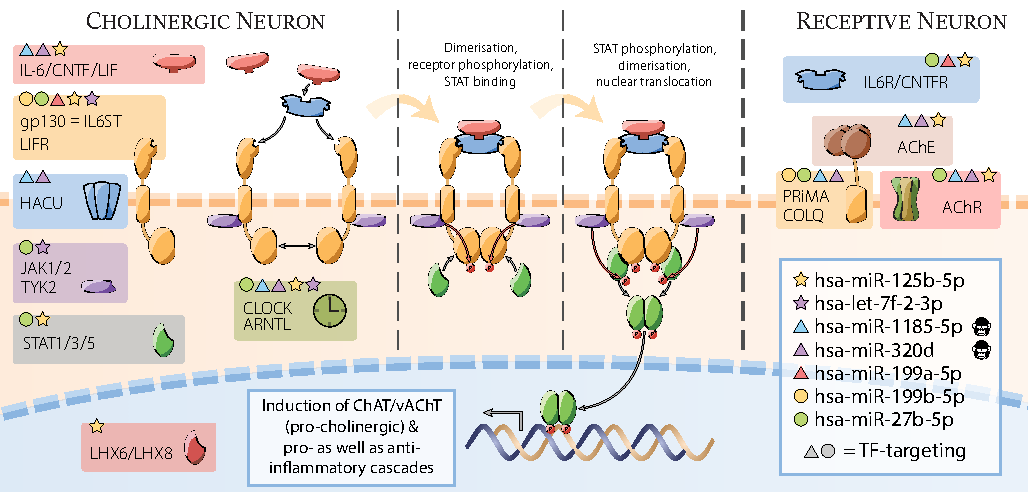
\includegraphics[width=\textwidth]{figures/neurokine}
\caption[The Cholinergic/Neurokine miRNA Interface.]{\textbf{The Cholinergic/Neurokine miRNA Interface.} The neurokines, such as CNTF, LIF, and IL-6, signal through a combination of soluble and membrane-bound receptors. Activation of a transmembrane neurokine receptor is usually followed by JAK recruitment and phosphorylation, and successively by STAT activation and translocation to the nucleus. Gp130-family neurokine, cholinergic, and circadian signalling pathways are controlled by primate-specific and evolutionarily conserved miRNAs. miRNA targeting of individual genes (indicated by coloured symbols) yields complex transcriptional interactions. Several miRNAs directly targeting the cholinergic pathway also target TFs controlling this pathway (circles and triangles).
\label{fig:neurokine}}
\end{figure}

A pivotal mediator of cholinergic/neurokine interaction, and of neurokine function in general, is the JAK/STAT pathway, which is immediately tied to gp130 activation. Importantly, JAK/STAT signalling is exclusive to neither cholinergic nor neurokine processes, but is critically important in both. Neurokines can activate tyrosine kinases JAK1/2 and TYK2, as well as STATs 1, 3, 5A, and 5B.\cite{Rawlings2004} Which of these leads to pro-cholinergic differentiation of neurons is still unclear and an interesting topic for further research.  Some work has been done on the distinction of effects between different members of the JAK and STAT families, mainly in immune cells. For instance, STAT1 activation in phagocytic monocytes leads to differentiation towards the M1 type pro-inflammatory macrophage, while STAT3 activation favours the generation of anti-inflammatory M2 type macrophages.\cite{Wang2014} The broad expression and wide-reaching functionalities of the JAK/STAT pathway bring with them an important caveat of all matters they were implicated in in the course of this dissertation, particularly in regard to gene ontology analyses: due to their importance in many processes in mammalian cells, they may be overrepresented in annotation, for instance in the ontology catalogues, such that these harbour an implicit bias for finding associations to JAK/STAT-related processes. Although there are measures in place in the analysis process that are supposed to suppress false identification, e.g. the weighing in R/topGO, there is no way of guaranteeing the absence of false positives in these results. However, since JAK/STAT mechanisms were implied with high frequency and in various independent analyses, there is a high level of confidence in their relevance to the studied phenomena.    

Neurokines are implicated in a range of diseases that have previously been associated with cholinergic systems and their dysfunction, particularly in the context of neuroinflammation, and particularly regarding IL-6. Whether this is a result of research bias, or of IL-6 actually being more relevant for disease processes, cannot at the moment be determined. There have been recent investigations of neurokine participation in AD,\cite{Pasquin2015,Baazaoui2018} SCZ,\cite{Chase2016,Girgis2018} BD,\cite{Goldsmith2016,Lu2019,Wiener2019} and stroke.\cite{Kang2012,Kang2013,Bustamante2014,Armstead2019} Thus, the establishment of LA-N-2 and LA-N-5 as human neuronal models of cholinergic/neurokine interaction can serve as a platform for further studies of the molecular mechanistic properties of this interaction and the evaluation of therapeutic interference in these systems (see also Section \ref{sec:discussion:therapy}).
 
%Dantzer complementarity between long and short range communication
%paracrine, endocrine, LIF induces catecholaminergic-to-cholinergic switch

%broadly acting vs specific mir families

%\subsection{Tissue Specificity of Small RNA Species} \label{sec:discussion:tissue}
%Another matter touched upon frequently in this dissertation

\subsection{Molecular Biology of Feedforward Loops}
Small RNA feedforward loops are a mechanistically feasible epigenetic controller of transcription,\cite{Cora2017} and the existence of biologically relevant FFLs has been convincingly shown.\cite{Lee2017} However, this evidence is still anecdotal, and thus, quantitative estimations of the extent of this phenomenon cannot with certainty be made. Hypothetically, feedforward loops affect a significant portion of all miRNA$\to$gene relationships, as can be seen in the FFL module analysis in Section \ref{sec:stroke:ffl}. Intriguingly, tRF$\to$gene feedforward loops (with a miRNA-like mechanism) are predicted in significantly smaller numbers. The stroke-relevant genes identified in Section \ref{sec:stroke:mrna} are involved in 3.5\% of miRNA FFLs (681 FFLs) and 11\% of tRF FFLs (21 FFLs). Thus, the low number of identified tRF-FFLs in stroke is not a stroke-specific observation, but rather a consequence of a low number of tRF-FFLs overall. Whether this is a result of the still inaccurate prediction or a real difference between these two smRNA species cannot be answered by my analyses. It is, however, an interesting question for future research. 

Hypothetically, if the low number of tRF-FFLs is not an artefact, but rather a representation of real epigenetic state, the question then arises, »What may the reason for this discrepancy be?« Generally observed, tRF$\to$gene interaction is present and not significantly less so than miRNA$\to$gene interaction, for instance in the FFL module analysis in Section \ref{sec:stroke:ffl}. For comparison, the network that is the basis for FFL analysis in Figure \ref{fig:cd14-ffl-modules} contains 481 miRNAs and 344 tRFs, but 681 miRNA-FFLs and only 21 tRF-FFLs. This discrepancy may carry biological significance, and two possible explanations come to mind: 1) tRFs may preferentially target genes that represent the ultimate stage of gene expression, and show less direct tRF$\to$TF interaction; or 2) tRFs show tRF$\to$gene and tRF$\to$TF interactions in similar extent as miRNAs, but the target sets do not overlap, i.e., targeted non-TF transcripts and TF transcripts do not form meaningful FFLs in the case of tRF targeting.

To determine the most likely answer based on my data, I calculated the ratio of smRNA$\to$TF to smRNA$\to$gene (excluding TFs) interactions for both smRNA species in the raw FFL network data of Figure \ref{fig:cd14-ffl-modules}. The ratio was similar in both species, around 10\% (miRNAs: 10.95\%, 6491 / 59\,269; tRFs: 9.37\%, 17\,542 / 187\,124), indicating that assumption \#1 may not hold. It follows that miRNAs and tRFs target TFs and non-TF genes in comparable amounts, but that the targeting in the case of miRNAs shows significantly more overlap between TFs and non-TF genes, leading to significantly more FFLs, in agreement with hypothesis \#2. This argument is only strengthened by the fact that the absolute number of tRF$\to$gene interactions was significantly higher as compared to miRNA$\to$gene (as a result of the score-based thresholding procedure in miRNA analysis).

Another aspect of FFL theory is the coherence of loops. While there are feasible roles for coherent as well as incoherent smRNA:TF:gene loops, their implications may diverge depending on the cellular context. Just looking at summary statistics, there is an implied difference between the two smRNA species: while miRNAs in the majority are down-regulated, tRFs in the majority are up-regulated (see Figure \ref{fig:stroke-de-tsne}). Combined with the preferential down-regulation of mRNA and the putative antagonistic role of both smRNA species, the general role of tRFs agrees with coherent FFLs, while the general role of miRNAs seems incoherent. Computing coherence on an individual FFL level indeed shows a high number of incoherent FFLs among all miRNA FFLs, mainly of the type »all down-regulated« (Figure \ref{fig:ffl-coherence}). Likewise, all 21 detected tRF FFLs were of the type »incoherent«. However, due to the very low number of tRF FFLs, this finding in all likelihood is not representative. The few detected tRF FFLs may also be false positives.

\begin{figure}
\centering
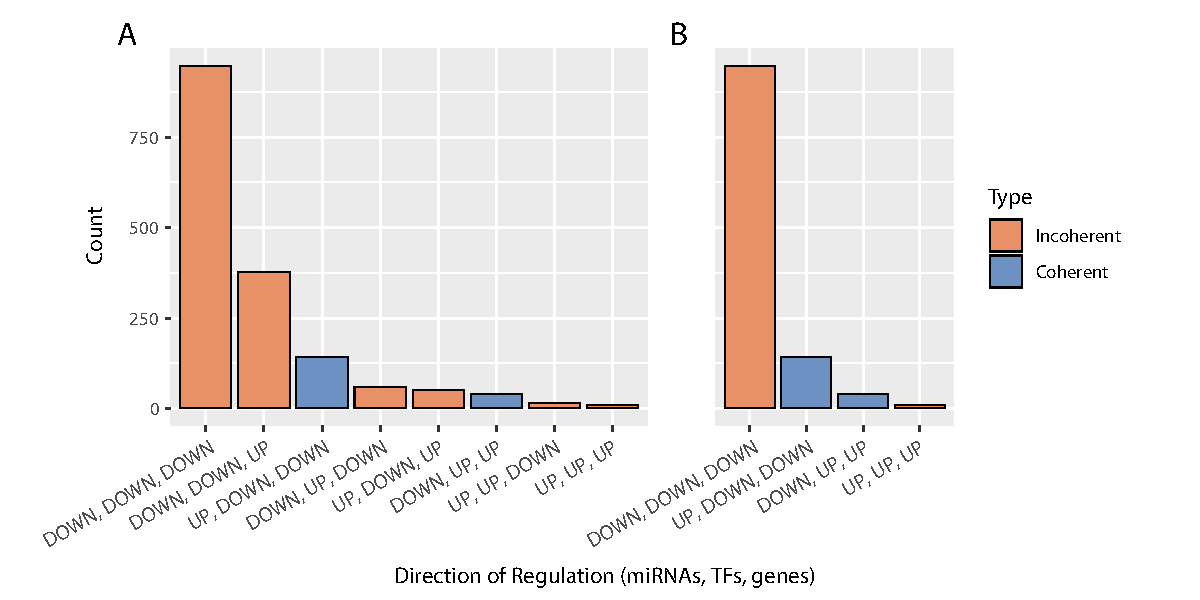
\includegraphics[width=\textwidth]{figures/ffl-coherence}
\caption[Coherence of miRNA Feedforward Loops.]{\textbf{Coherence of miRNA Feedforward Loops.} Individual FFLs were classified based on the direction of regulation of each of their components (miRNAs, TFs, and non-TF genes) in the blood of stroke patients, as determined via RNA-seq. Barplots represent the count of each class of FFL, colour denotes coherence. Incoherent FFLs dominate quantitatively. \textbf{A)} Barplot of all possible types of FFLs. \textbf{B)} Barplots of FFLs only with coherent TF$\to$gene relationships (both either up- or down-regulated). 
\label{fig:ffl-coherence}}
\end{figure}

Regardless of their individual biological significance, FFLs can be used as a tool to gain insight on transcriptional processes. FFLs may identify tightly connected processes, and allow stratification of large data, which is one of the main problems in descriptive bioinformatics. The approach shown in Section \ref{sec:stroke:ffl} is an attempt at dimensionality reduction that retains as much of the original data structure as possible, while allowing human interpretation. As is demonstrated by the comparison between GO analyses on the whole set of data and the individual clusters as defined by FFL analysis (Figure \ref{fig:gsoap-ffl}), the latter allows deeper insight into the biological processes affected by stroke through its increased resolution.

In this manner, the most pathologically pertinent coding transcripts in the blood of stroke victims were identified and classified, as well as their associations with biological processes involved in pathogenesis of or response to the infarction. The main biological pathways identified in this context are involved in immunity and inflammation, cell death, regulation of transcription, STAT signalling, lipid metabolism, and blood vessel integrity. A comparison between annotated FFL modules and t-SNE visualisation of module GO terms summarises the implications drawn from this bioinformatically supported clinical study (Figure \ref{fig:ffl-gsoap-comp}). Of note, the number of molecules comprising each module correlates with the number of GO terms identified for the respective module, as seen by the comparison between the largest module (two) and the smallest modules (three and four). This can be explained by the comparison of the number of DE genes in each module and the absolute number of genes making up any GO term (i.e., the \emph{successes}). Hypergeometric enrichment p-values are dependent on the size of the set of successes, and thus, the likelihood of identifying a large (i.e., less specific) GO term with a comparatively small number of test set genes is very low, which is not the case for smaller, highly specific GO terms. Consequently, larger modules (test sets) have available to them a larger number of GO terms that can potentially be enriched.

Comparing the topography between Figure \ref{fig:ffl-gsoap-comp} A and B, the location of most modules appears as a mirror image. This could be interpreted as a confirmation of the general feasibility of the approach: the similarity of transcripts as determined by their participation in closely related FFLs is paralleled by the similarity of module GO terms as determined by the genes shared between the GO terms. However, a significant difference between the two visualisations seems the  central position of module one in Figure \ref{fig:ffl-gsoap-comp}\,B, which may indicate a central relevance of module one transcripts in the studied processes. Indeed, module one GO terms appear to function as a nucleation point for related terms from the other modules (central cluster of Figure \ref{fig:ffl-gsoap-comp}\,B), which may be used as an indicator of a focus point for further studies.

\begin{figure}
\centering
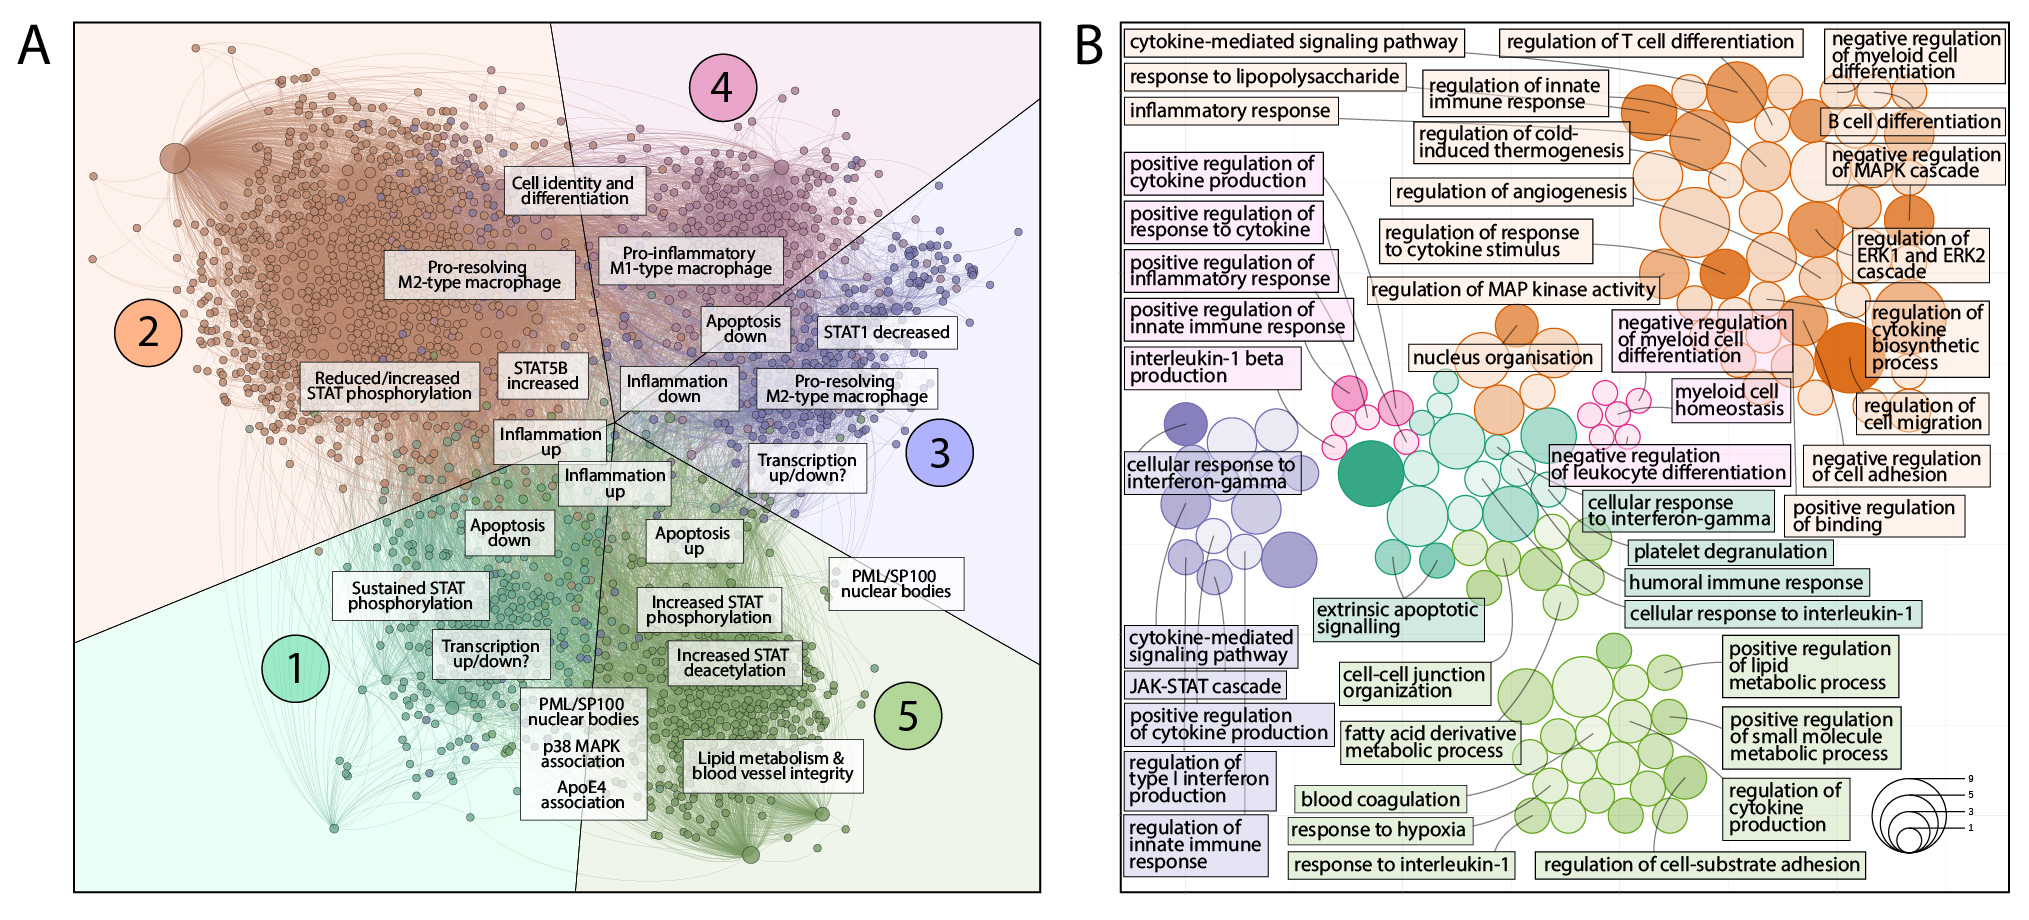
\includegraphics[width=\textwidth]{figures/ffl-gsoap-comp}
\caption[Comparison of Annotated Feedforward Loop Network and t-SNE Visualisation of Module GO Terms.]{\textbf{Comparison of Annotated Feedforward Loop Network and t-SNE Visualisation of Module GO Terms.} \textbf{A)} Reproduction of Figure \ref{fig:cd14-ffl-annot}, colours have been adapted to allow module comparison between \textbf{A} and \textbf{B}. Displayed is the network of all CD14$^+$-specific FFLs, stratified into five modules, and overlaid with module-specific GO analysis results. \textbf{B)} Reproduction of Figure \ref{fig:gsoap-ffl}\,B. Displayed is the t-SNE-based visualisation of all module-specific GO terms from the CD14$^+$ FFL-network (\textbf{A}), coloured by module. The distance between nodes is based on amount of shared genes between terms, depth of colour represents significance level, size of node represents number of genes in term.
\label{fig:ffl-gsoap-comp}}
\end{figure}

There are several lines of investigation that could be based on the present results: 1) As described above, the cluster surrounding module one GO terms could be dissected as to the implications of the genes relevant to these terms. These genes may represent a »cooperative set«, which mediates between the distinct modules and their influences on the biological processes in question. As such, it may be interesting to »zoom in« into the network of only those genes defining this central cluster, to identify pathways sitting at the epicentre of transcriptional response to stroke.

2) Feedforward loops as an abstract classification method may be helpful in the differentiation of inductive versus repressive behaviours of single TF$\to$gene relationships. As discussed several times in the course of this dissertation (see e.g. Section \ref{sec:discussion:ffl}), the current comprehensive data on TF$\to$gene interaction does not allow prediction of the direction of regulatory influence of the TF over the gene. Even in manually collected data, such as TRANSFAC, the interaction of TF and gene is often described in a »yes/no« fashion, with the added limitation of tissue-specific information that is not easily transferred. This is mainly owed to the fact that most TF:gene interactions are found via binding assays such as \ac{chip} sequencing and related variants. The combination of smRNA:TF:gene FFLs with interventional experiments (i.e., yielding regulatory output) may serve as methodical support to determine the direction of regulation in individual TF$\to$gene interactions. The application of FFLs (from prediction or web-available datasets) to experiments (also from web-available datasets) may aid in detecting regulatory circuits, and a meta-analysis of these circuits across multiple different experiments may be used to calculate likelihood data of positive or negative regulatory interaction between any TF and gene. Such an approach may be a cost-effective data-mining alternative to painstaking single-experiment molecular biology.

3) Similarly, FFLs can aid in the classification of small RNA species and their families and sub-families in a functional manner. The participation in FFLs from a comprehensive dataset can be mathematically transformed into a similarity- or distance-matrix, and the information so gained on relationships among smRNAs can be used for the stratification and analysis of relationships between individual smRNAs. This classification can serve as an independent comparative dataset, complementing the traditional strata derived from phylogenetic studies.

4) There is need for the development of statistical frameworks in the analysis of feedforward loops. In particular, a measure for the relative importance of each FFL in a network would be helpful for the dissemination of the network and its functions. Possible components of a mathematical description of significance in this setting may be the differential expression of FFL components, the strength of the interaction between FFL components, or network-specific parameters such as centrality. A formal definition of such an »importance measure« is not a trivial task and will require extensive comparison and validation.

\newpage
%!TEX root = ../dissertation.tex
\section{Small RNA Therapeutics and Pharmacology} \label{sec:discussion:therapy}
\subsection{Interactions Between Small Molecule Drugs and Small RNAs}
While we know a lot about the transcriptional effects of approved small molecule drugs, and likewise have learned much about the workings of miRNAs in regulating the transcriptome, the intersection between small molecule drug effects and miRNAs (and other small RNAs) \emph{in vivo} is still very current and ongoing research. There have been reports of miRNA regulation conveying drug resistance in single instances (mainly in cancer);\cite{Ma2010} for example, the deletion of the genomic locus containing the miR-125b gene led to an increased susceptibility of breast cancer patients to anthracylines.\cite{Climent2007} There have been attempts at comprehensively assessing the potential interaction spaces between drug- and miRNA-effects,\cite{Meng2016, Xie2019} however, these are limited to indirect comparison of the transcript spectra of drugs and miRNAs compared (»drug \textbf{A} influences expression of gene \textbf{B}, which is also influenced by miRNA \textbf{C}, so there may be interaction«), and text mining. Both examples are relatively crude estimations of possible interactions, feature a low resolution, and disregard tissue-specific effects and transcription factor interactions, both of which are elementary in the effects of most approved transcriptionally relevant drugs.\cite{Clayton2018}

While a majority of drug-miRNA interactions is still in the dark, it is feasible that miRNAs not only convey drug resistance, but may also play a part in the known effects of approved small molecule drugs, particularly those with known transcriptional effects. There have been single reports of miRNA perturbations upon treatment with antipsychotics such as halo"-per"-i"-dol, clozapine, and chlorpromazine, but those reports are seldom and remain descriptive.\cite{Gardiner2014} Clayton and colleagues have recently reviewed the role of miRNAs in \acf{gc} action.\cite{Clayton2018} They found that miRNAs modulate the biogenesis of GCs in the adrenal glands as well as cell responses to GCs. At least part of the effects of GCs in cell function, proliferation, and survival are conveyed via their regulation of miRNA expression. The GC receptor is regulated by miRNAs, such that a repression of the receptor by up-regulated miRNAs conveyed treatment resistance in leukaemias and asthma. In leukocytes, miR-155 down-regulation is an important aspect of GC-mediated suppression of inflammation; dexamethasone-mediated suppression of the response to \acf{lps} inhibited the up-regulation of miR-155 in primary macrophages, macrophage cell lines, spleen and liver cells of mice, and T cells of sepsis patients.\cite{Clayton2018} In our hands, dexamethasone prevented the up-regulation of the top six stroke-perturbed \acfp{trf} in murine RAW 264.7 macrophages \emph{in vitro}.\cite{Winek2020}

GCs also inhibit the expression of miR-101, which leads to impaired \acf{mapk} activation and subsequent suppression of inflammation. Resistance to GC-induced apoptosis in multiple myeloma has been associated with elevations of miR-221/222 and miR-125b. Paradoxically, GCs themselves increase the expression of miR-125b, which may constitute a negative feedback mechanism, partly via suppression of p53.\cite{Murray2013} Notably, members of the mir-10/199 families (see Section \ref{sec:cellculture:mir-go}) are closely intertwined with regulation of GC function. In addition to the aforementioned effects of miR-125b on GC action, miR-125a and miR-10b regulate GC synthesis via interaction with CYP11B1 and CYP11B2 (11-Deoxycorticosterone $\to$ Corticosterone $\to$ Aldosterone; 11-Deoxycortisol $\to$ Cortisol), whereas miR-199a is up-regulated by GC treatment of osteoblasts and conveys WNT pathway suppression, and miR-199a levels were found to be reduced in patients with Cushing's disease. Clayton \emph{et al.}\cite{Clayton2018} also identify major hurdles in the development of therapeutic strategies paying respect to miRNA involvement, which are congruent with my own assessment. The first refers to the complex biological role of small RNAs and the challenges it presents to bioinformatics: 

\begin{quote}
»How are functional interactions to be predicted with confidence, and how are subtle effects of individual miRNAs to be experimentally validated without the danger of confirmation bias? How are miRNA-mediated effects on biological processes to be identified and understood when they involve many-to-many rather than one-to-one interactions?«
\end{quote}

The second refers to the challenge in translating the biological knowledge so gained into effective treatment:

\begin{quote}
»Even where good therapeutic targets can be clearly identified, it remains to be seen whether a mimic or antagonist of a single miRNA species will be sufficient to exert therapeutic effects. If targeting more than one miRNA proves necessary, this will create additional barriers to development, in part because of the problem of predicting and mitigating off-target effects.«
\end{quote}

These questions imply that mimicking or antagonism of an endogenous miRNA (or multiple) may not be the most logical way of pursuing small RNA therapeutic applications, which will be addressed in the following section (\ref{sec:discussion:smrna-therapy}).

\subsection{Small RNAs as Pharmacological Agents} \label{sec:discussion:smrna-therapy}
Application of small oligonucleotides in therapy of human diseases is in the early stages of development. Theoretically, antisense oligonucleotides can, via their instrumentalisation of endogenous RNA interference machinery, silence virtually any gene in the human body, including non-coding genes. Thus, presuming an appropriate design strategy, synthetic oligonucleotides possess a broader spectrum than traditional small molecule drugs. Because of their chemical nature, i.e., high molecular weight and poly-ionised backbone, oligonucleotides cannot cross biological membranes via passive diffusion and therefore have to be delivered using advanced pharmaceutical formulations, most commonly, lipid nanoparticles (Figure \ref{fig:lipid}).\cite{Akhtar2007, Whitehead2009} Additionally, to circumvent recognition by the host defence system, e.g. by \acp{tlr}, the bases composing the oligonucleotide are often chemically modified. Common modifications include the 2'-O-methyl sugar modification, which prevents TLR7-mediated response, bridging between two sugar molecule carbon atoms (creating so-called »locked nucleic acids«), which fix the nucleotides in a specific steric position, and hybridisation to molecules such as cholesterol or polyethylene glycol, which can convey steric hindrance and even organ targeting properties.\cite{Whitehead2009}

\begin{figure}
\centering
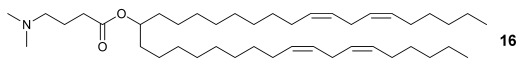
\includegraphics[width=.7\textwidth]{figures/mfig004}
\caption[siRNA Nanoparticle Lipid.]{\textbf{siRNA Nanoparticle Lipid.} (6Z ,9Z ,28Z ,31Z )-Heptatriaconta-6,9,28,31-tetraen-19-yl 4-(dimethylamino)butanoate. Image and caption from Jayaraman \emph{et al.}\cite{Jayaraman2012}
\label{fig:lipid}}
\end{figure}

Once they have reached the cytoplasm of the target cell, therapeutic antisense oligonucleotides can load into the \acf{risc} and convey translational suppression similar to endogenous molecules such as miRNAs and tRFs. Notably, and perhaps surprisingly, single-dose application of comparatively low doses of synthetic oligonucleotides can continuously suppress target mRNA synthesis, and consequently protein expression, over a period of months.\cite{Raal2020} The most advanced lipid nanoparticles are composed of ionisable amino lipids that self-assemble into particles of the size of approximately \SI{100}{\nano\metre} when mixed with polyanionic oligonucleotides (i.e., the drug molecules).\cite{Akhtar2007} The dual function of these amino lipids is 1) to interact with drug molecules via ion-ion interaction, forming the delivery particles and 2) to allow the drug molecules to escape from endosomes after endocytosis by the target cell. Through developments in the last two decades, these particles have reached a therapeutic index suitable for human therapy.\cite{Jayaraman2012, Raal2020}

The first FDA-approved antisense drug was afovirsen, approved in 1991 for use in human papillomavirus treatment, targeting the \emph{E2} gene implicated in virus replication. However, afovirsen and the Bcl2-antisense oblimersen failed their clinical trials. It took several more years for the first synthetic oligonucleotide to be approved for human treatment: fomivirsen, also a blocker of viral RNA, for the local treatment of HIV-associated cytomegalovirus retinitis, was approved in 1998.\cite{Piascik1999} It has since been retracted, but several others are currently approved for treatment: mipomersen for the treatment of familial hypercholesterinaemia, defibrotide for treatment of veno-occlusive liver disease, eteplirsen and golodirsen for treatment of Duchenne muscular atrophy, pegaptanib for age-related macular atrophy, nusinersen for treatment of spinal muscular atrophy, inotersen for the treatment of heritable transthyretin-mediated amyloidosis, and volanesorsen for treatment of hypertriglyceridaemia, familial chylomicronaemia syndrome and familial partial lipodystrophy.\cite{Sharad2019, Wang2020} A fascinating case is the personalised oligonucleotide (named milasen) for therapy of the rare neurodegenerative condition »Batten's disease«, which has been specifically designed for the patient Mila Makovec based on a sequencing of her genome, and which modifies the splicing of the mutated \emph{MSFD8} gene identified as causal in her affliction.\cite{Kim2019} It can be described as a repurposed version of nusinersen, featuring the same backbone and sugar chemistry modifications, but adapted to target the splicing of \emph{MSFD8} instead of \emph{SMN2} mRNA.

Notably, extant antisense approaches are characterised by their high specificity for an affected organ (liver, eye) and a bias for rare diseases, many of them previously untreatable. The organ specificity can be explained by the delivery aspect: due to their chemical nature, they are most effective if applied to the organ directly (eye) or if they are hybridised to a targeting molecule. The discovery of hybridisation of an oligonucleotide to N-acetylgalactosamine, which specifically binds to asialo-glycoprotein receptors expressed by hepatocytes, has led to a surge in candidates for the treatment of liver-associated diseases (Figure \ref{fig:pathophys-porphyria}).\cite{Wang2020} In addition, capillary endothelia in most tissues do not easily allow the passage of particles larger than \SI{5}{\nano\metre}; notable exceptions are tissues containing sinusoidal endothelia, particularly the bone marrow, liver, and spleen.\cite{Gullotti2009, Hassanshahi2019} The remainder of extant approaches are explained largely by the orphan status of the targeted diseases, facilitating approval. Most pipeline drugs are being developed in the fields of oncology and neurology; as of late, RNA antisense therapeutics seem to have reached the point of profitability.\cite{Wang2020} 

\begin{figure}[ht]
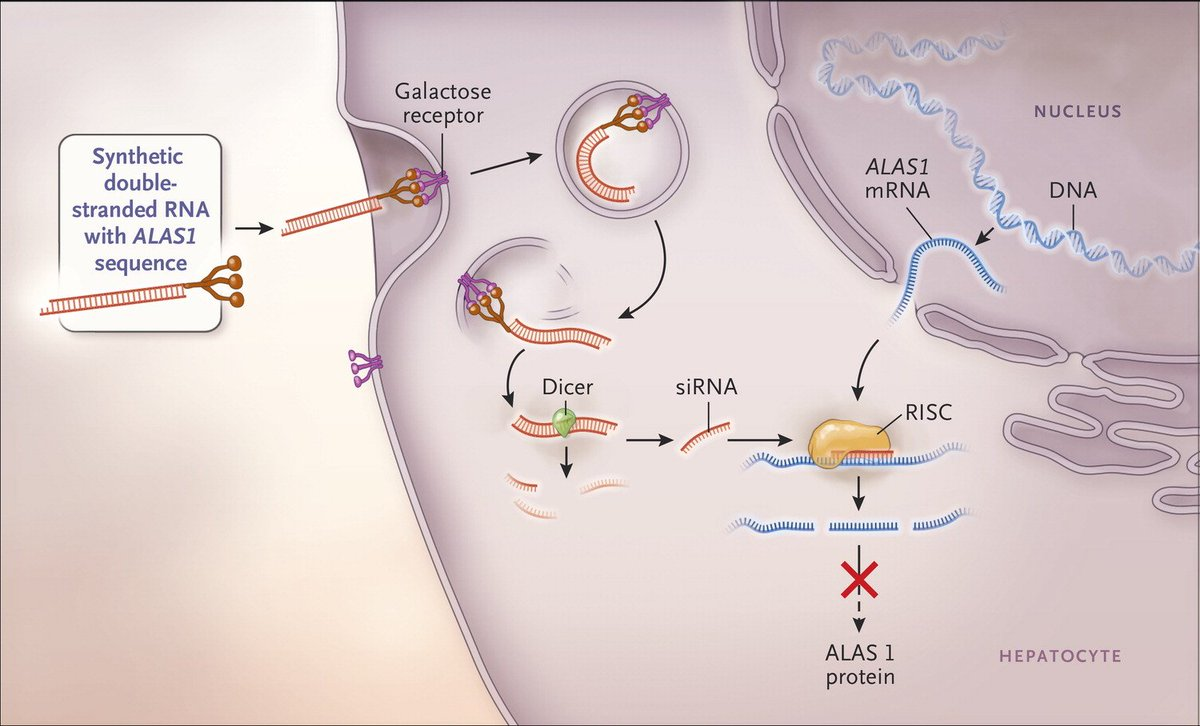
\includegraphics[width=\textwidth]{figures/pathophys-porphyria-therapy-sirna-nejm-original}
\caption[The Mechanism of Small Interfering RNA (siRNA) Therapy.]{\textbf{The Mechanism of Small Interfering RNA (siRNA) Therapy.} Synthetic double-stranded RNA containing an ALAS1-specific sequence is derivatized with N-acetylgalactosamine to target the asialoorosomucoid (galactose) receptor, which is expressed nearly exclusively on hepatocytes. Within the hepatocyte, the RNA is processed into approximately 20-bp fragments by a cellular enzyme (dicer), and then separated into single strands. The strand that is complementary to ALAS1 (the guide strand) binds to cellular ALAS1 messenger RNA (mRNA) and enters the RNA-induced silencing complex (RISC), where the new double-stranded RNA is cleaved by a group of factors that include argonaute, a ribonuclease. The result is a reduction in the level of delta ALA synthase 1 protein and decreased production of ALA. Image and caption by Dr. Gerald Diaz.\cite{Diaz2018}
\label{fig:pathophys-porphyria}}
\end{figure}

Another notable common characteristic of antisense therapeutics on the market or in the pipeline is the monogenetic or pseudo-monogenetic nature of the targeted diseases. For instance, in neurology, phase III pipeline candidates include IONIS-HTT$_{Rx}$ for treatment of Huntington's disease, and tofersen for treatment of SOD1-driven amyotrophic lateral sclerosis. Both diseases are characterised by a clear understanding of how changes in single transcripts cause pathology, and thus are easily accessible to the design of an antisense sequence. Inclisiran, also known as ALN-PCSsc, has recently successfully completed phase II trial for the treatment of familial hypercholesterinaemia.\cite{Raal2020} Its target is the \ac{pcsk} mRNA, reduction of which leads to a reduction in \ac{ldl} particles. Similarly to other liver-targeted oligonucleotides, inclisiran is hybridised to triantennary N-acetylgalactosamine carbohydrates, conveying liver-specific receptor-mediated endocytosis. The encapsulating lipid nanoparticles utilise the aminolipid DLin-MC3-DMA (see Figure \ref{fig:lipid}).\cite{Jayaraman2012} Inclisiran has been shown to significantly alleviate familial hyper"-chol"-es"-ter"-in"-aemia (\ac{ldl}-levels reduced by approximately 40\%) via only bi-annual subcutaneous application.\cite{Frank-Kamenetsky2008, Fitzgerald2014, Fitzgerald2017, Raal2020}

The use of single-target oligonucleotides parallels the leitmotif of modern medicinal chemistry: creating drugs with as little off-target effects as possible, to be able to tightly control the biological effects of the drug while simultaneously preventing adverse effects. Due to their extreme target specificity caused by mRNA complementarity, antisense oligonucleotides mainly cause adverse effects via their application (e.g., local effects at the subcutaneous injection site) or the compounds needed to facilitate their delivery (e.g., the lipid nanoparticles). Considering the very infrequent application as compared to other subcutaneous therapeutics, the general adverse effect risk of antisense therapy can be considered low.\cite{Raal2020}

The main problem in antisense therapy in its current state is the limitation to easily accessible compartments and the single-target nature of the drugs. All diseases featured in this dissertation (compare Section \ref{sec:intro:diseases} and Chapters 3 \& 4) are known for their polygenetic or poly-factorial nature, and thus, monogenetic therapeutic approaches are bound to fail. Additionally, psychiatric diseases present the major delivery hurdle of the blood-brain-barrier, and possibly pose advanced delivery problems such as single affected CNS cell types. Traditional small molecule therapeutics in psychiatric disease are known for their extreme range of target molecules. Most are derived from chlorpromazine, an artefact of antihistamine discovery synthesis, and are notorious for their targeting of multiple classes of neurotransmitter receptors. Impressively, second generation antipsychotics, which generally are seen as an improvement over the first generation of chlorpromazine-type antipsychotics, often present a more extensive and complex receptor profile, contrary to the specificity leitmotif of medicinal chemistry.

Translation of the knowledge of these dynamics in psychiatric diseases to antisense oligonucleotide therapy is the biggest hurdle for the design of adequate drug molecules. As opposed to small molecule drugs (high throughput screening of synthetic derivative molecules), serendipity is all but impossible in the case of antisense drugs, which are comprised of combinations of only four principal building blocks, as opposed to thousands of different chemical moieties, but a greater combinatorial multitude of possible molecules: $4^n$, with the common length of 22 nt, yields approximately 17.6 trillion individual molecules. The iterative screening of all possible combinations of the four bases in common high-throughput assays would quickly exceed experimental capacities and would lead to uneconomic development costs, particularly if seeking a multi-target oligonucleotide. Thus, bioinformatic predictions of suitable candidate molecules to be tested are necessary for efficient and economic screening of drug candidates for any given application, as well as for the prior identification of suitable combinations of target molecules in any given disease.

The dissertation here presented provides an infrastructure for these analysis steps (Chapter 2) as well as examples for high-prevalence diseases (Chapters 3 \& 4). Integrative transcriptomics analyses can serve as tools for the identification of pertinent pathways in pathogenesis as well as for the development of oligonucleotides with multi-target behaviour that enables synergistic effects in therapy and an imitation of multiple-target small molecule drug behaviour. Priorities in these analyses can be set to reflect the researchers' focus; for instance, an analytical prior could bias the search towards pharmacologically interesting targets that are so far inaccessible to small molecule drugs, such as IRF5 in inflammation (see Section \ref{sec:stroke:ffl-cd14}).\cite{Almuttaqi2019} Multi-target oligonucleotides can follow two principal design strategies: the mimicking or antagonising of extant endogenous smRNA molecules, such as miRNAs, or the de-novo creation of oligonucleotides based on complementarity to predefined target transcripts. The former method is more likely to be efficacious in a short time frame, but brings with it the risk of generating a plethora of adverse effects, because the target profiles of miRNAs are mostly very broad, tissue specific, and not entirely clear yet. De-novo design, on the other hand, theoretically allows the creation of defined target populations without off-target effects. The human genome is known, and thus, sequences can be generated that are complementary only to the target RNA molecules, without any other hits across the genome. However, since not all mechanistic aspects of RNA interference are clear (canonical versus non-canonical binding, bridging, wobble), not all complementary oligonucleotides are similarly effective. Thus, candidate molecules require thorough testing. This brings attention to another important limitation in de-novo design of oligonucleotide drugs: due to the differences in species genomes, these molecules cannot be comprehensively tested in animal models, particularly in rodents. Safety considerations thus should have utmost priority in clinical evaluation of such molecules. Studies of these phenomena have led to the new subfields of genocompatibility and toxicogenomics.\cite{Akhtar2007}

In immunology, hybridisation of oligonucleotide drugs to immune cell-specific receptor ligands could be used to convey a cell-type specificity akin to current liver-specific approaches. Many transcription factors (TFs) show highly context-dependent activities,\cite{Hamada2020} and thus, a combination of TF specificity conveyed by the oligonucleotide and cell type specificity conveyed by a hybridisation partner may allow context-dependent intervention. For instance, ligands specific for CD4$^+$ cells could be used to target oligonucleotides to T helper cells, targeting relevant TFs such as NF-$\upkappa$B or STATs to modify the inflammatory reflex; oligonucleotides hybridised to CD14$^+$-targeting ligands could be utilised to interfere with monocyte responses, e.g. after stroke. Due to the trafficking of immune cells between brain and periphery, therapy of diseases with neuroinflammatory components could be accessible through the much easier peripheral (e.g., subcutaneous) application. Considering the accessibility of different tissues to standard parenteral application routes, the most promising strategies are targeting of immune cells circulating in the blood, or stationary in the spleen, both of which are relatively permissible to nanoparticles,\cite{Gullotti2009} and, in limited fashion, also lymph nodes, which can accommodate particle sizes between 10 and \SI{100}{\nano\metre}.\cite{Schudel2019} A knockdown of few select monocyte-specific transcripts could be used to drive differentiation towards the pro-resolving M2-type macrophage population,\cite{Panizzi2010} possibly breaking the vicious cycle of protracted inflammation. Co-targeting of cholinergic and neurokine transcripts may interfere more causally in pathogenesis of diseases with cholinergic participation than current single-target small molecule approaches.

%sexual differences